% !TEX root = ../../main.tex
\subsection{Mutation}

One of the ingredients for evolution to take place is the constant appearance
of genetic variability. After all, the raw material for evolution to act on is
the appearance of new mutations in the population. This is what we will model
now for our one-locus two-allele case. We will think of mutations between both
alleles $A$ and $a$ as a simple first-order chemical reaction of the form
\begin{equation}
  A \xrightleftharpoons[\mu_{a A}]
  {\,\mu_{A a}\,} a,
\end{equation}
where $\mu_{A a}$ is the mutation rate from $A$ to $a$ and 
$\mu_{a A}$ is the mutation rate from $a$ to $A$. A useful way to
interpret the mutation rate is as the probability of switching allele per unit
time. That means that on a small time window $\Dt$ a single organism has a
probability of switching from $A$ to $a$ of
\begin{equation}
  P(A \rightarrow a \mid \Dt) = \mu_{A a} \Dt, \quad 
  \text{for } \Dt \ll \mu_{Aa}.
\end{equation}
What this implies is that for this small time window every organism carrying
allele $A$ flips a coin with probability $\mu_{A a} \Dt$ of getting
heads. If the outcome of the coin is indeed heads, the allele is mutated,
otherwise it remains the same. So when writing a differential equation to model
this phenomena we must multiply the number of organisms by the mutation rate.
This results in a differential equation for the change in number of organisms
carrying $A$ of the form
\begin{equation}
  \dt{N_A} = 
  \underbrace{- \mu_{A a} N_A(t)}_{\text{loss } A \rightarrow a}
  \underbrace{- \mu_{a A} N_a(t)}_{\text{gain } a \rightarrow A},
\end{equation}
where, as indicated, we must account for number of organisms that ``exit'' the
$A$ allele state by mutating to $a$, and the number of organisms that ``enter''
the state by mutating from $a$ to $A$. We can write an equivalent equation for
$N_a$ where the signs would be simply flipped since every time an organism is
lost from allele $A$ it must be gained in allele $a$, and vice versa. This
implies that for this case where there is only mutation $N\tot$ does not change
over time since the number of organisms is assumed to be conserved.

Let us now write the dynamics that we actually care about, that is the allele
frequency $x(t)$. This takes the form
\begin{equation}
  \dt{x} = \dt{}\left( {N_A \over N\tot} \right) = {1 \over N\tot} \dt{N_A},
\end{equation}
where we took $N\tot$ out of the derivative since for this case we said it
doesn't change over time. Substituting the dynamics of $N_A$ and using the
definition of the allele frequency we obtain
\begin{equation}
  \dt{x} = - \mu_{A a} x + \mu_{a A} (1 - x),
  \label{eq_mutation_ode}
\end{equation}
where we again suppressed the time dependence for notation simplicity. This
equation can also be solved analytically, but before getting to that solution
let's take a look at the steady state value. After all we know that these are
deterministic dynamics so the allele fraction will reach a unique point. The
steady state results in
\begin{equation}
  \mu_{A a} x_{ss} = \mu_{a A} (1 - x_{ss}),
\end{equation}
where $x_{ss}$ indicates that it is the steady state allele frequency. If we
now solve for $x_{ss}$ this results in
\begin{equation}
  x = {\mu_{a A} \over \mu_{a A} + \mu_{A a}}.
\end{equation}
So the equilibrium allele frequency for this case is given by the rate of how
often strains mutate from $a$ to $A$ divided by the sum of those rates. That
means that in the limit where it is much more likely to mutate from $a$ to $A$,
i.e. $\mu_{a A} \gg \mu_{A a}$ the allele frequency goes
to one, i.e. allele $A$ will go into fixation. The opposite would be true for a
much larger mutation rate from $A$ to $a$.

Now let's go ahead and solve the actual dynamics. \eref{eq_mutation_ode} is an
ordinary differential equation that can again be solved by separation of
variables. This is
\begin{equation}
  \int {dx \over - \mu_{A a} x + \mu_{a A} (1 - x)} = 
  \int dt.
\end{equation}
Evaluating the integrals results in
\begin{equation}
  -{1 \over \mu_{a A} + \mu_{A a}}
  \ln \left( \mu_{A a} x - \mu_{a A} (1 - x) \right) =
  t + C,
  \label{eq_mutation_int}
\end{equation}
where $C$ is an integration constant. Using again the initial condition where
$x(t=0) = x_o$ we have that
\begin{equation}
  C =  -{1 \over \mu_{a A} + \mu_{A a}}
  \ln \left( \mu_{A a} x_o - \mu_{a A} (1 - x_o) \right).
\end{equation}
Using this result we can rewrite \eref{eq_mutation_int} as
\begin{equation}
  -{1 \over \mu_{a A} + \mu_{A a}}
  \ln \left( { \mu_{A a} x - \mu_{a A} (1 - x)
    \over
  \mu_{A a} x_o - \mu_{a A} (1 - x_o)} \right) = t.
\end{equation}
Exponentiating both sides gives
\begin{equation}
  \left( { \mu_{A a} x - \mu_{a A} (1 - x)
    \over
  \mu_{A a} x_o - \mu_{a A} (1 - x_o)} \right)^{
    -{1 \over \mu_{a A} + \mu_{A a}}} = \E^t
\end{equation}
If we now elevate both sides to the $\mu_{a A} + \mu_{A\rightarrow
a}$ power we obtain
\begin{equation}
  \left( { \mu_{A a} x - \mu_{a A} (1 - x)
    \over
  \mu_{A a} x_o - \mu_{a A} (1 - x_o)} \right) =
  \E^{- (\mu_{a A} + \mu_{A a}) t}.
\end{equation}
We can now solve for $x$ and after a little bit of algebra we find that
\begin{equation}
  x(t) = {\mu_{a A} 
  \over 
  \mu_{a A} + \mu_{A a}} -
  {\left[  
  \mu_{a A} -
  (\mu_{a A} + \mu_{A a}) x_o
  \right] 
  \E^{- (\mu_{a A} + \mu_{A a}) t}.
  \over
  \mu_{a A} + \mu_{A a}}.
\end{equation}
A little tricky solution, but we can easily see that in the limit when $t
\rightarrow \infty$ the second term on the right hand side goes to zero,
leaving behind the steady state solution we found before. \fref{fig_01_02}
shows the dynamics for different ratios of the mutation rates. We can see that
as expected the allele frequency converges to the steady state value we
derived.

\begin{figure}[h!]
	\centering 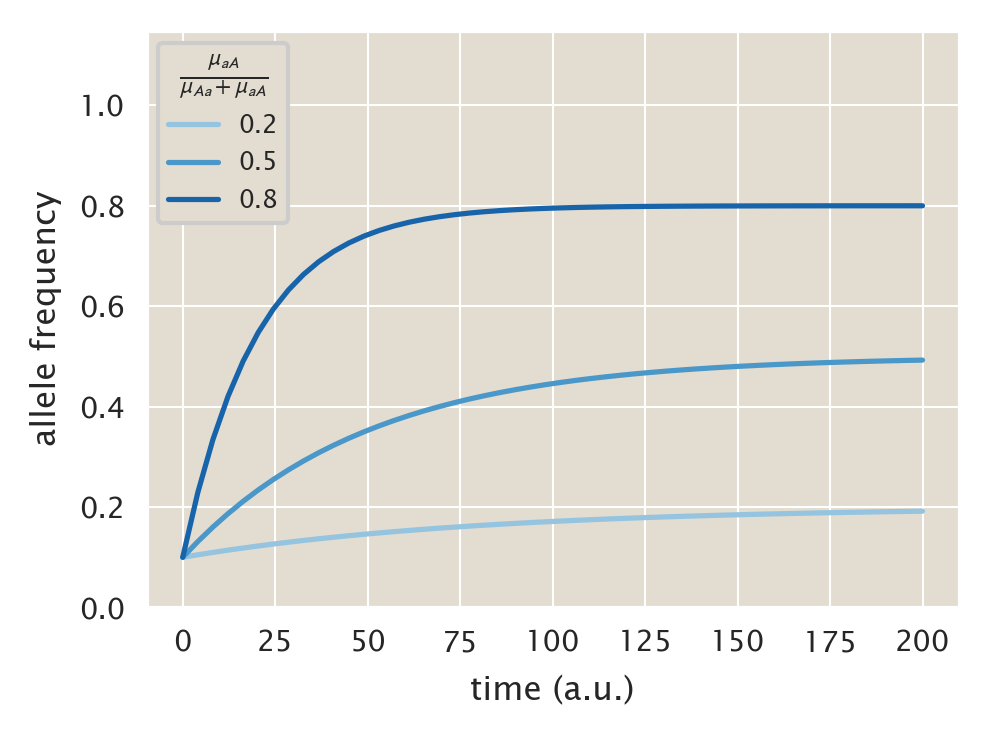
\includegraphics
  {../fig/deterministic_evo/01_02_deterministic_mut.png}
	\caption{\textbf{Allele frequency for mutation only}. The different curves
	show allele frequency dynamics for a one-locus two-allele system mutating
	between both alleles. The steady state allele frequency is set by the ratio
	of the mutation rates.}
  \label{fig_01_02}
\end{figure}

\subsubsection{Mutation-Selection Balance}

Now that we have modeled two of the three forces we will be using throughout
the notes let us try to put them together. Since both selection and mutation
are directional deterministic forces we can easily add them together for our
allele frequency dynamics and still obtain a deterministic answer. The dynamics
for our single-locus two-allele system subject to both selection and mutation
are given by the sum of the dynamics for each case. This is
\begin{equation}
  \dt{x} = s x (1 - x) - \mu_{Aa} x + \mu_{aA} (1 - x).
  \label{eq_sel_mut}
\end{equation}
This linear ODE can be solved analytically as you can asses yourself by plugin
this equation into a symbolic math package such as Mathematica or Sympy. The
problem is that the solution is not intuitive with a bunch of tangents and
arctangents that make it very difficult to look at. Nevertheless we can still
gain intuition from \eref{eq_sel_mut}. An interesting setting to analyze is the
case where one of the alleles, let's say $a$ is deleterious, i.e. $s < 0$. If
that were the case our results from \secref{sec_selection} tell us that natural
selection would remove this allele from the population. But if mutation keeps
bringing the allele back over and over again, there should be a balance between
mutation and selection. This is a plausible scenario if we think of allele $A$
as a functional protein, and $a$ is a coarse-grained state of all
non-functional proteins for example. To compute this equilibrium we need to
compute the steady state for \eref{eq_sel_mut} as
\begin{equation}
  0 = s x_{ss}^2 + (\mu_{Aa} + \mu_{aA} - s) x_{ss} - \mu_{aA},
\end{equation}
where we already expanded the terms and group by powers of $x_ss$, the steady
state allele frequency. The roots of this quadratic equation are given by
\begin{equation}
  x_{ss} = {(s - \mu_{Aa} - \mu_{aA}) \pm 
    \sqrt{(\mu_{Aa} - \mu_{aA} - s)^2 + 4 s \mu_{aA}}
    \over 2s}.
\end{equation}
If again we take $a$ as a coarse-grained state for a non-functional gene we can
assume that reversing the mutation to the functional allele is very unlikely,
therefore we can set $\mu_{aA} \approx 0$. This results in
\begin{equation}
  x_{ss} = {(s - \mu_{Aa}) \mp (s - \mu_{Aa}) \over 2s}.
\end{equation}
The resulting two possible steady states are then
\begin{equation}
  x_{ss1} = 0, \quad x_{ss2} = 1 - {\mu_{Aa} \over s}.
\end{equation}
The first case shows that if allele $A$ were to go extinct it would stay as
such. The more interesting and relevant case is the second root. This shows
that the allele frequency decreases from the fixation value 1 depending on the
relative strengths of mutation and selection.